\documentclass[a4paper]{article}
\usepackage[utf8]{inputenc}
\usepackage[T1]{fontenc}
\usepackage[intlimits]{amsmath}
\usepackage{amsfonts}
\usepackage{amssymb}
\usepackage[export]{adjustbox}
\usepackage{graphicx}
\setlength{\parindent}{0pt}
\usepackage[left=1in, right=1in, top=1in, bottom=1in]{geometry}
\usepackage{float}
\usepackage{multicol}
\usepackage{listings}
\usepackage{xcolor}
\usepackage{cancel}
\usepackage{bm}
\usepackage{hyperref}
\setcounter{tocdepth}{1}
\usepackage[titletoc]{appendix}
\hypersetup{
	colorlinks=true,
	linkcolor=blue,
	filecolor=blue,
	urlcolor=blue,
}

\begin{document}
	
	\Huge\textbf{Mechanism Startup Calculator}
	\newline
	\LARGE AMB Calculator
	
	\vspace{0.5cm}
	\normalsize
	
	This calculator is used to simulate the start-up response of a motorized mechanism.\\
	
	A DC motor can be represented by the following electrical circuit:
	
	\begin{figure}[H]
		\centering
		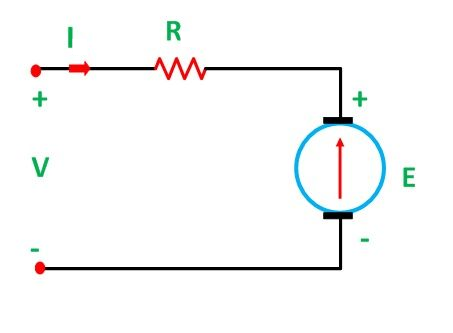
\includegraphics[width=0.7\linewidth]{dc_motor.png}
	\end{figure}
	
	The voltage in this circuit can be represented as:
	
	\begin{equation} \label{kirchoff}
		V = I R - E
	\end{equation}
	\\
	where $ V $ is the voltage applied to the motor, $ I $ is the current drawn by the motor, $ R $ is the armature resistance, and $ E $ is the back-emf generated by the motor. The back-emf is linearly related to the motor speed according to a constant $ k_B $, so:
	
	\begin{equation} \label{back-emf}
		E = k_B \cdot \omega_{motor}
	\end{equation}
	\\
	Plugging (\ref{back-emf}) into (\ref{kirchoff}) and solving for the motor current gives:
	
	\begin{equation}
		I = \frac{V - k_B \cdot \omega_{motor}}{R}
	\end{equation}
	\\
	This current can then be limited according to current limit set in the motor controller.\\
	
	The torque generated by the motor $ T_{motor} $ is proportional to the armature current according to a constant $ k_T $, so:
	
	\begin{equation}
		T_{motor} = k_T \cdot I
	\end{equation}
	\newpage
	
	The speed of the motor $ \omega_{motor} $ is $ G $ times faster than the mechanism speed $ \omega $, where $ G $ is the gear ratio between the two. The mechanism torque $ T $ is also $ G $ times greater than the motor torque $ T_{motor} $.
	
	\begin{equation}
		T = k_T G \cdot I \qquad\qquad
		I = \frac{V - k_B G \cdot \omega}{R}
	\end{equation}
	\\
	According to Newton's second law, the angular acceleration of the system $ \alpha $ is proportional to the sum of the torques on the system $ \Sigma T $ and the mechanism's moment of inertial $ J $:
	
	\begin{equation}
		\Sigma T = T - T_{load} = J \cdot \alpha
	\end{equation}
	\\
	The load torque can be represented by the load force times the applied radius:
	
	\begin{equation}
		T_{load} = F_{load} \cdot r
	\end{equation}
	\\
	And the moment of inertia can be approximated as that of a point mass $ m $ at radius $ r $:
	
	\begin{equation}
		J \approx m \cdot r^2
	\end{equation}
	\\
	Combining these equations gives an expression for the angular acceleration of the system:
	
	\begin{equation}
		\alpha = \frac{T - T_{load}}{J} = \frac{T - F_{load} \cdot r}{m r^2}
	\end{equation}
	\\
	The angular acceleration can then be used to find the change in angular velocity $ \omega $ over one timestep $ dt $, which can be used to find the change in position $ \theta $:
	
	\begin{equation}
		\omega_{t+dt} = \omega_t + \alpha \cdot dt \qquad\qquad
		\theta_{t+dt} = \theta_t + \omega_t \cdot dt + \tfrac{1}{2} \alpha_t \cdot {dt}^2
	\end{equation}
	\\
	Starting with $ \theta_0 = 0 $ and $ \omega_0 = 0 $, we can simulate the start up response of the system one timestep at a time, until either the target position/velocity or maximum time is reached.

	
	
	
	
	
\end{document}